\documentclass[10pt]{article}
\usepackage[paperwidth=8.27in,paperheight=11.69in,margin=0.62in]{geometry}
\usepackage[T1]{fontenc}
\usepackage{lmodern}
\usepackage{xcolor}
\usepackage{tikz}
\usetikzlibrary{arrows.meta,positioning,fit,calc}
\usepackage[most]{tcolorbox}
\usepackage{listings}
\usepackage{amsmath,amssymb}
\usepackage{microtype}
\usepackage{enumitem}
\pagestyle{empty}

\definecolor{ink}{HTML}{263238}
\definecolor{muted}{HTML}{607D8B}
\definecolor{blue}{HTML}{377DFF}
\definecolor{bluepale}{HTML}{EEF4FF}
\definecolor{teal}{HTML}{159D8C}
\definecolor{tealpale}{HTML}{EAF8F5}
\definecolor{amber}{HTML}{D88B16}
\definecolor{amberpale}{HTML}{FFF6E6}
\definecolor{line}{HTML}{DCE5EA}
\definecolor{codebg}{HTML}{F6F8FA}

\color{ink}
\setlength{\parindent}{0pt}
\setlength{\parskip}{3pt}
\setlist{nosep,leftmargin=1.2em}
\newcommand{\lean}{\textsf{Lean 4}}
\newcommand{\tagpill}[2]{\tikz[baseline=(x.base)]\node[rounded corners=3pt,fill=#1,inner xsep=5pt,inner ysep=2pt,text=ink,font=\sffamily\scriptsize\bfseries] (x) {#2};}
\newcommand{\sectiontitle}[1]{\vspace{2pt}{\sffamily\bfseries\large #1}\par\vspace{4pt}}

\lstdefinelanguage{Lean}{
  morekeywords={theorem,where,by,apply,exact,obtain,rintro,fun,cases,with,let,in,if,then,else},
  morekeywords=[2]{Type,Sort,CompleteSemilatticeSup,ENat,ENNReal},
  morecomment=[l]{--}, morecomment=[s]{/-}{-/},
  sensitive=true
}
\lstset{language=Lean,basicstyle=\ttfamily\fontsize{7.4}{9}\selectfont,
  keywordstyle=\color{blue}\bfseries,keywordstyle=[2]\color{teal},
  commentstyle=\color{muted}\itshape,showstringspaces=false,
  columns=fullflexible,keepspaces=true,aboveskip=4pt,belowskip=2pt}

\newtcolorbox{softbox}[2][]{enhanced,boxrule=0.6pt,arc=5pt,
  colback=#2,colframe=line,left=8pt,right=8pt,top=6pt,bottom=6pt,#1}

\begin{document}

% PAGE 1
{\sffamily\fontsize{23}{26}\selectfont\bfseries From duplicate proofs to a reusable lemma}\par
\vspace{3pt}
{\sffamily\color{muted}A small, reviewable mathlib contribution pattern}\hfill
\tagpill{bluepale}{PATTERN}\;\tagpill{tealpale}{EXTRACT}\;\tagpill{amberpale}{REUSE}

\vspace{13pt}
\begin{center}
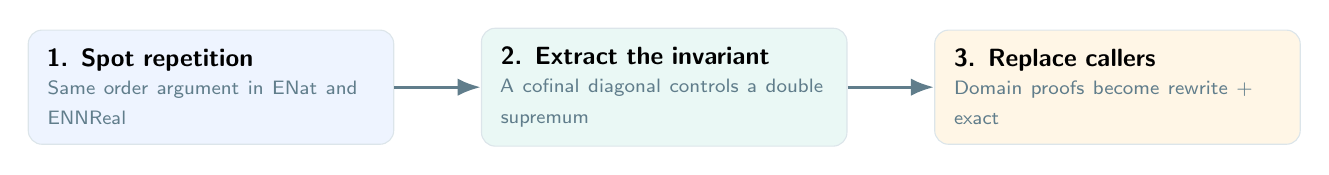
\begin{tikzpicture}[node distance=7mm and 11mm,>=Latex,
  card/.style={draw=line,rounded corners=5pt,text width=4.15cm,minimum height=1.12cm,
    align=left,inner sep=7pt,font=\sffamily\small},
  flow/.style={->,very thick,color=muted}]
  \node[card,fill=bluepale] (a) {\textbf{1. Spot repetition}\\[-1pt]\color{muted}\scriptsize Same order argument in ENat and ENNReal};
  \node[card,fill=tealpale,right=of a] (b) {\textbf{2. Extract the invariant}\\[-1pt]\color{muted}\scriptsize A cofinal diagonal controls a double supremum};
  \node[card,fill=amberpale,right=of b] (c) {\textbf{3. Replace callers}\\[-1pt]\color{muted}\scriptsize Domain proofs become rewrite + exact};
  \draw[flow] (a) -- (b); \draw[flow] (b) -- (c);
\end{tikzpicture}
\end{center}

\vspace{8pt}
\sectiontitle{The duplicated shape}
\begin{softbox}{codebg}
\begin{minipage}[t]{0.47\linewidth}
\tagpill{bluepale}{ENat.iSup\_add\_iSup}
\begin{lstlisting}
refine le_antisymm ?_ ?_
refine iSup_add_iSup_le fun i j => ?_
rcases h i j with <k, hk>
exact le_iSup_of_le k hk
\end{lstlisting}
\end{minipage}\hfill
\begin{minipage}[t]{0.47\linewidth}
\tagpill{bluepale}{ENNReal.iSup\_add\_iSup}
\begin{lstlisting}
refine le_antisymm ?_ ?_
refine iSup_add_iSup_le fun i j => ?_
rcases h i j with <k, hk>
exact le_iSup_of_le k hk
\end{lstlisting}
\end{minipage}
\end{softbox}

\vspace{8pt}
\sectiontitle{The weakest common statement}
\begin{softbox}{tealpale}
\begin{lstlisting}
@[to_dual iInf2_eq_diagonal]
theorem iSup2_eq_diagonal
    {alpha : Type*} {iota : Sort*} [CompleteSemilatticeSup alpha]
    (f : iota -> iota -> alpha)
    (h : forall i j, exists k, f i j <= f k k) :
    (iSup i, iSup j, f i j) = iSup k, f k k := by
  ...
\end{lstlisting}
\end{softbox}

\vspace{9pt}
\begin{center}
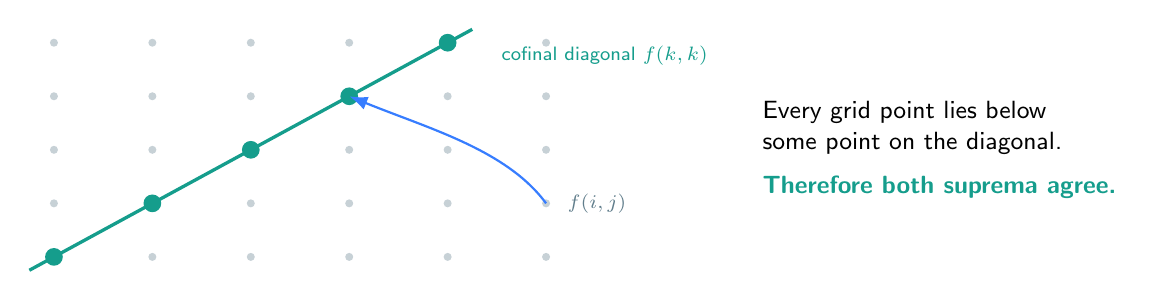
\begin{tikzpicture}[x=1.25cm,y=0.68cm,>=Latex]
  \foreach \x in {0,...,5} {\foreach \y in {0,...,4} {
    \fill[muted!35] (\x,\y) circle (1.45pt);
  }}
  \foreach \k in {0,...,4} {\fill[teal] (\k,\k) circle (3.2pt);}
  \draw[teal,very thick] (-.25,-.25)--(4.25,4.25);
  \draw[blue,->,thick] (5,1) .. controls (4.6,2.0) and (3.8,2.4) .. (3,3);
  \node[font=\sffamily\scriptsize,text=muted,anchor=west] at (5.12,1) {$f(i,j)$};
  \node[font=\sffamily\scriptsize,text=teal,anchor=west] at (4.45,3.75) {cofinal diagonal $f(k,k)$};
  \node[font=\sffamily\small,align=left,anchor=west] at (7.1,2.0) {
    Every grid point lies below\\some point on the diagonal.\\[5pt]
    \color{teal}\bfseries Therefore both suprema agree.};
\end{tikzpicture}
\end{center}

\vfill
{\color{muted}\scriptsize\sffamily Contribution shape: one generic order lemma $\rightarrow$ two shorter callers $\rightarrow$ no new framework.}

\newpage

% PAGE 2
{\sffamily\fontsize{23}{26}\selectfont\bfseries Proof map in Lean 4}\par
\vspace{3pt}
{\sffamily\color{muted}Two inequalities, then immediate reuse}\hfill\tagpill{tealpale}{MACHINE-CHECKED}

\vspace{12pt}
\sectiontitle{Goal}
\begin{softbox}{codebg}
\centering
$\displaystyle \Big(\sup_i\sup_j f(i,j)\Big)=\sup_k f(k,k)$
\qquad under \qquad
$\displaystyle \forall i\,j,\ \exists k,\ f(i,j)\le f(k,k)$.
\end{softbox}

\vspace{10pt}
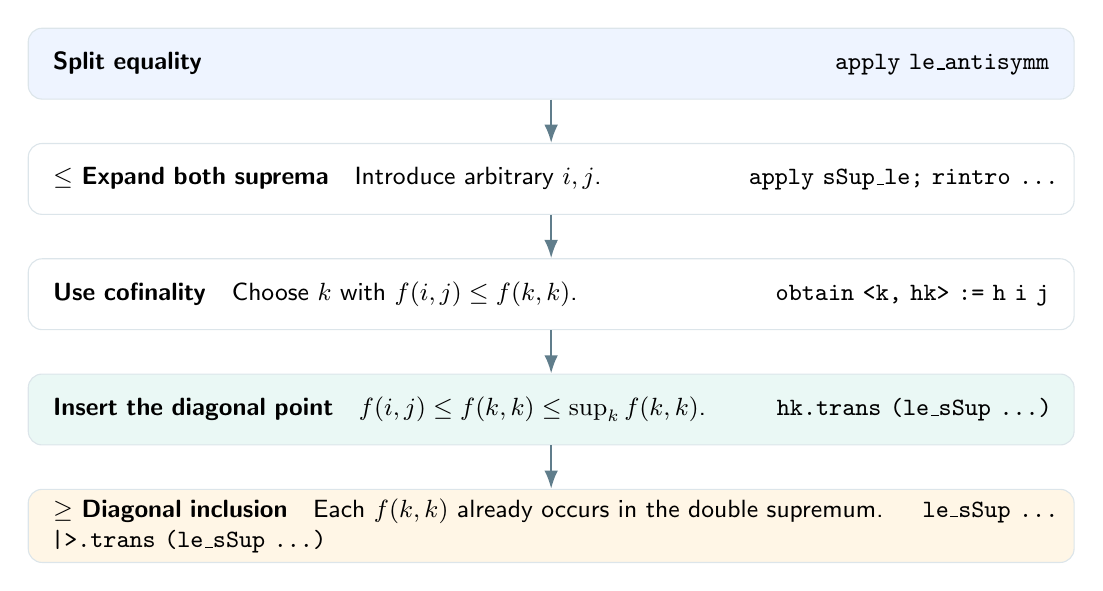
\begin{tikzpicture}[node distance=5.5mm,>=Latex,
 proofstep/.style={draw=line,rounded corners=5pt,minimum height=9mm,text width=12.65cm,
   inner xsep=9pt,align=left,font=\sffamily\small},
 arr/.style={->,thick,color=muted}]
 \node[proofstep,fill=bluepale] (s0) {\textbf{Split equality}\hfill\texttt{apply le\_antisymm}};
 \node[proofstep,fill=white,below=of s0] (s1) {\textbf{$\le$ Expand both suprema}\quad Introduce arbitrary $i,j$.\hfill\texttt{apply sSup\_le; rintro ...}};
 \node[proofstep,fill=white,below=of s1] (s2) {\textbf{Use cofinality}\quad Choose $k$ with $f(i,j)\le f(k,k)$.\hfill\texttt{obtain <k, hk> := h i j}};
 \node[proofstep,fill=tealpale,below=of s2] (s3) {\textbf{Insert the diagonal point}\quad $f(i,j)\le f(k,k)\le\sup_k f(k,k)$.\hfill\texttt{hk.trans (le\_sSup ...)}};
 \node[proofstep,fill=amberpale,below=of s3] (s4) {\textbf{$\ge$ Diagonal inclusion}\quad Each $f(k,k)$ already occurs in the double supremum.\hfill\texttt{le\_sSup ... |>.trans (le\_sSup ...)}};
 \foreach \a/\b in {s0/s1,s1/s2,s2/s3,s3/s4} \draw[arr] (\a)--(\b);
\end{tikzpicture}

\vspace{11pt}
\sectiontitle{Caller reduction}
\begin{softbox}{amberpale}
\begin{minipage}[t]{0.48\linewidth}
{\sffamily\bfseries Before}\par
\begin{lstlisting}
cases isEmpty_or_nonempty iota
. simp only [iSup_of_empty, ...]
. refine le_antisymm ?_ ?_
  refine iSup_add_iSup_le fun i j => ?_
  rcases h i j with <k, hk>
  exact le_iSup_of_le k hk
\end{lstlisting}
\end{minipage}\hfill
\begin{minipage}[t]{0.48\linewidth}
{\sffamily\bfseries After}\par
\begin{lstlisting}
cases isEmpty_or_nonempty iota
. simp
. simp_rw [ENat.iSup_add, ENat.add_iSup]
  exact iSup2_eq_diagonal
    (fun i j => f i + g j) h
\end{lstlisting}
\end{minipage}
\end{softbox}

\vspace{10pt}
\sectiontitle{Why this is upstream-friendly}
\begin{center}

\begin{tikzpicture}[node distance=7mm and 8mm,
 item/.style={draw=line,rounded corners=12pt,fill=white,minimum width=3.35cm,
 minimum height=1cm,font=\sffamily\small\bfseries,align=center}]
 \node[item] (a) {Weak assumption\\[-2pt]\scriptsize\color{muted}CompleteSemilatticeSup};
 \node[item,right=of a] (b) {Predictable name\\[-2pt]\scriptsize\color{muted}iSup2\_eq\_iSup\_diagonal};
 \node[item,right=of b] (c) {Visible reuse\\[-2pt]\scriptsize\color{muted}ENat + ENNReal};
 \node[item,right=of c] (d) {Dual for free\\[-2pt]\scriptsize\color{muted}iInf2\_eq\_iInf\_diagonal};
\end{tikzpicture}
\end{center}

\vspace{10pt}
\begin{softbox}{bluepale}
{\sffamily\bfseries Review checklist}\hfill
\tagpill{white}{generic}\quad\tagpill{white}{discoverable}\quad\tagpill{white}{2 callers}\quad\tagpill{white}{build + lint}
\end{softbox}

\vfill
{\color{muted}\scriptsize\sffamily Source artifact: \texttt{RequestProject/Main.lean}. The formal theorem and both replacement callers compile without \texttt{sorry}.}



\newpage

% PAGE 3
{\sffamily\fontsize{23}{26}\selectfont\bfseries Big idea: duplicate proofs are failed factorisations}\par
\vspace{3pt}
{\sffamily\color{muted}The repeated code is evidence that one mathematical morphism has not yet been named}\hfill\tagpill{tealpale}{STRUCTURE}

\vspace{11pt}
\begin{center}
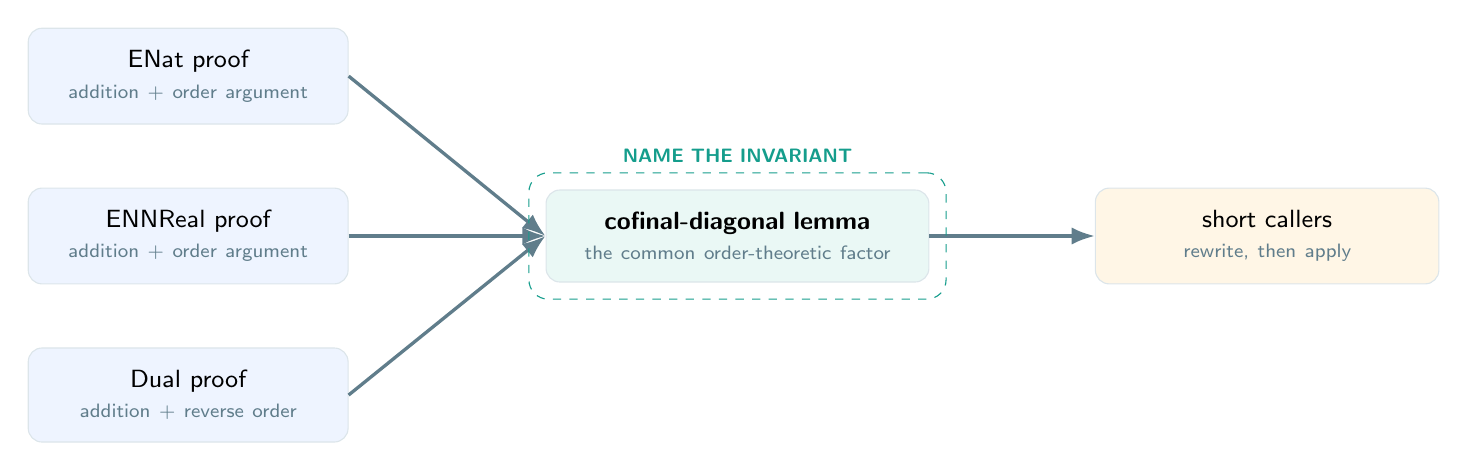
\begin{tikzpicture}[node distance=8mm and 12mm,>=Latex,
  box/.style={draw=line,rounded corners=5pt,align=center,inner sep=8pt,font=\sffamily\small},
  arrow/.style={->,very thick,color=muted}]
  \node[box,fill=bluepale,text width=3.5cm] (p1) {ENat proof\\\scriptsize\color{muted}addition + order argument};
  \node[box,fill=bluepale,text width=3.5cm,below=of p1] (p2) {ENNReal proof\\\scriptsize\color{muted}addition + order argument};
  \node[box,fill=bluepale,text width=3.5cm,below=of p2] (p3) {Dual proof\\\scriptsize\color{muted}addition + reverse order};
  \node[box,fill=tealpale,text width=4.3cm,right=25mm of p2] (core) {\textbf{cofinal-diagonal lemma}\\\scriptsize\color{muted}the common order-theoretic factor};
  \node[box,fill=amberpale,text width=3.8cm,right=21mm of core] (clients) {short callers\\\scriptsize\color{muted}rewrite, then apply};
  \draw[arrow] (p1.east)--(core.west);
  \draw[arrow] (p2.east)--(core.west);
  \draw[arrow] (p3.east)--(core.west);
  \draw[arrow] (core)--(clients);
  \node[draw=teal,dashed,rounded corners=7pt,fit=(core),inner sep=6pt,
    label={[font=\sffamily\scriptsize\bfseries,text=teal]above:NAME THE INVARIANT}] {};
\end{tikzpicture}
\end{center}

\vspace{8pt}
\sectiontitle{The abstraction ladder}
\begin{center}
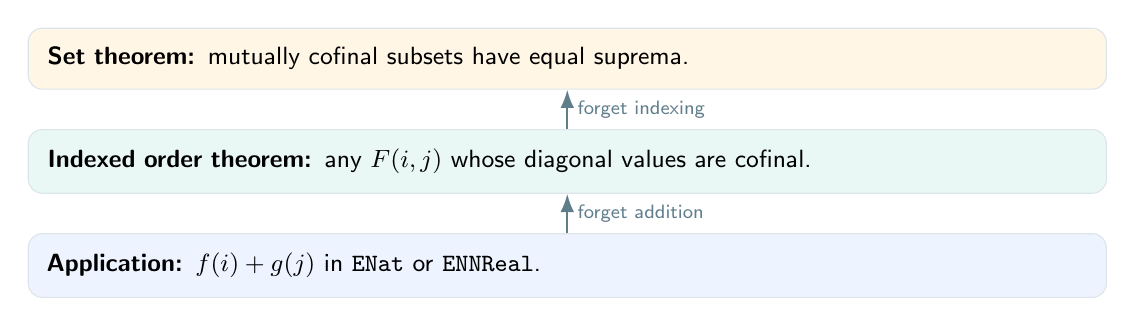
\begin{tikzpicture}[node distance=5mm,>=Latex,
 level/.style={draw=line,rounded corners=5pt,text width=13.2cm,inner sep=7pt,font=\sffamily\small},
 up/.style={->,thick,color=muted}]
 \node[level,fill=bluepale] (l1) {\textbf{Application:} $f(i)+g(j)$ in \texttt{ENat} or \texttt{ENNReal}.};
 \node[level,fill=tealpale,above=of l1] (l2) {\textbf{Indexed order theorem:} any $F(i,j)$ whose diagonal values are cofinal.};
 \node[level,fill=amberpale,above=of l2] (l3) {\textbf{Set theorem:} mutually cofinal subsets have equal suprema.};
 \draw[up] (l1)--node[right,font=\sffamily\scriptsize,text=muted]{forget addition} (l2);
 \draw[up] (l2)--node[right,font=\sffamily\scriptsize,text=muted]{forget indexing} (l3);
\end{tikzpicture}
\end{center}

\vspace{8pt}
\begin{softbox}{tealpale}
{\sffamily\bfseries The design rule: abstract exactly as far as the reuse evidence supports.}\par
A good lemma forgets accidental data (addition, number type, local names) while retaining the
minimal structure needed by the proof (here, a complete supremum semilattice and cofinality).
Going farther can be mathematically elegant, but without callers it increases API and review cost.
\end{softbox}

\vspace{8pt}
\sectiontitle{Cool fact: a two-dimensional supremum can be one-dimensional}
\begin{softbox}{amberpale}
The whole grid may look larger than its diagonal, yet cofinality makes the diagonal a
\emph{lossless compression}: it sees every value up to domination. This is not a cardinality claim;
it is a claim about what the supremum can detect.
\end{softbox}

\vfill
{\color{muted}\scriptsize\sffamily Structural smell: when proofs differ only in the ambient type, look for the universal order argument they instantiate.}

\newpage

% PAGE 4
{\sffamily\fontsize{23}{26}\selectfont\bfseries Three analogies for cofinality}\par
\vspace{3pt}
{\sffamily\color{muted}Different pictures of the same invariant: maxima care about reach, not enumeration}\hfill\tagpill{amberpale}{INTUITION}

\vspace{12pt}
\begin{center}
\begin{tikzpicture}[node distance=7mm and 8mm,>=Latex,
 cardx/.style={draw=line,rounded corners=6pt,text width=4.15cm,minimum height=5.3cm,align=left,inner sep=8pt,font=\sffamily\small}]
 \node[cardx,fill=bluepale] (sky) {\textbf{1. Skyline sensors}\\[4pt]
   \begin{tikzpicture}[x=.45cm,y=.38cm]
    \foreach \x/\h in {0/2,1/4,2/1.5,3/3,4/5,5/2.5,6/4.5} {\draw[muted,very thick] (\x,0)--(\x,\h);\fill[muted] (\x,\h) circle (1.5pt);}
    \draw[teal,very thick] (-.2,5)--(6.2,5);
   \end{tikzpicture}\\[4pt]
   \scriptsize A selected sensor network suffices if every omitted reading is no higher than some selected reading. The skyline maximum is unchanged.};
 \node[cardx,fill=tealpale,right=of sky] (train) {\textbf{2. Express stops}\\[4pt]
   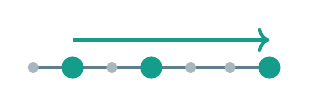
\begin{tikzpicture}[x=.5cm]
    \draw[muted,thick] (0,0)--(6,0);
    \foreach \x in {0,...,6} \fill[muted!55] (\x,0) circle (2pt);
    \foreach \x in {1,3,6} \fill[teal] (\x,0) circle (4pt);
    \draw[teal,->,very thick] (1,.35)--(3,.35)--(6,.35);
   \end{tikzpicture}\\[7pt]
   \scriptsize An express route can ignore local stops while still reaching arbitrarily far along the line. A tail property observed on the express route controls the full route.};
 \node[cardx,fill=amberpale,right=of train] (sync) {\textbf{3. Synchronising clocks}\\[4pt]
   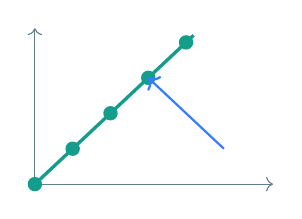
\begin{tikzpicture}[x=.48cm,y=.45cm]
    \draw[->,muted] (0,0)--(6.3,0); \draw[->,muted] (0,0)--(0,4.4);
    \foreach \k in {0,...,4} {\fill[teal] (\k,\k) circle (2.6pt);}
    \draw[teal,very thick] (0,0)--(4.2,4.2);
    \draw[blue,->,thick] (5,1)--(3,3);
   \end{tikzpicture}\\[1pt]
   \scriptsize Two independent indices $(i,j)$ can be advanced to one common time $k$. Directedness supplies the synchronisation point.};
\end{tikzpicture}
\end{center}

\vspace{10pt}
\begin{softbox}{bluepale}
{\sffamily\bfseries What all three analogies preserve}\par
Not the individual points, their order, or their number. They preserve one universal question:
\emph{is every discarded value bounded by a retained value?} If yes, taking a supremum cannot tell
the full family from the retained cofinal subfamily.
\end{softbox}

\vspace{9pt}
\begin{softbox}{amberpale}
{\sffamily\bfseries Important non-analogy}\par
``Diagonal'' here does \textbf{not} mean Cantor's diagonal argument. No contradiction or
self-reference is involved. It is the ordinary map $k\mapsto(k,k)$, used to replace two indices
by one common upper stage.
\end{softbox}

\vspace{9pt}
\sectiontitle{A reusable mental test}
\begin{center}

\begin{tikzpicture}[node distance=7mm and 9mm,>=Latex,
 q/.style={draw=line,rounded corners=10pt,fill=white,minimum height=9mm,text width=3.7cm,align=center,font=\sffamily\small\bfseries},
 a/.style={->,thick,color=muted}]
 \node[q] (x) {Which values are discarded?};
 \node[q,right=of x] (y) {Does a retained value dominate each one?};
 \node[q,right=of y,fill=tealpale] (z) {Then the supremum is preserved.};
 \draw[a] (x)--(y); \draw[a] (y)--(z);
\end{tikzpicture}
\end{center}

\vfill
{\color{muted}\scriptsize\sffamily Cofinality is ``coverage at the top'': it forgets low-level enumeration while retaining all information visible to a supremum.}

\newpage

% PAGE 5
{\sffamily\fontsize{23}{26}\selectfont\bfseries The category-theory pattern}\par
\vspace{3pt}
{\sffamily\color{muted}The order lemma is a thin-category shadow of cofinality and colimit invariance}\hfill\tagpill{bluepale}{CATEGORY VIEW}

\vspace{11pt}
\begin{softbox}{bluepale}
{\sffamily\bfseries Dictionary}\par
\begin{center}
\begin{tabular}{lll}
\textbf{Order theory} & \textbf{Category theory} & \textbf{In this example}\\[2pt]
preorder & thin category & one arrow $x\to y$ iff $x\le y$\\
least upper bound & colimit of a diagram & $\sup_i f(i)$\\
cofinal subset/map & final functor & keep only enough indices\\
order dual & opposite category & supremum $\leftrightarrow$ infimum
\end{tabular}
\end{center}
\end{softbox}

\vspace{10pt}
\begin{center}
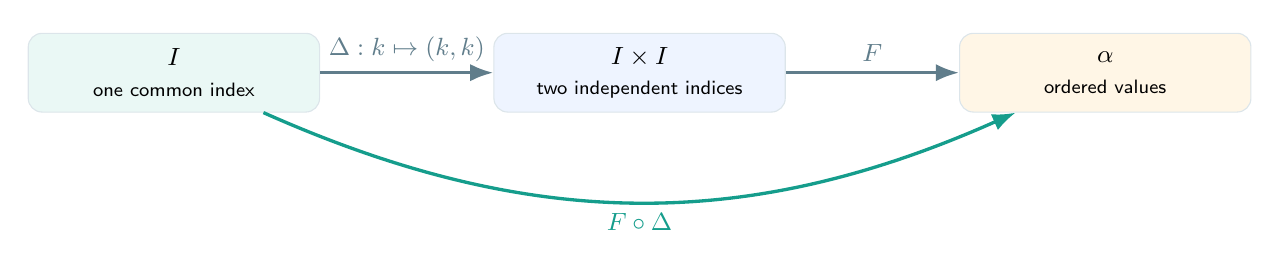
\begin{tikzpicture}[node distance=12mm and 22mm,>=Latex,
 obj/.style={draw=line,rounded corners=5pt,fill=white,minimum width=3.7cm,minimum height=1cm,align=center,font=\sffamily\small},
 fun/.style={->,very thick,color=muted}]
 \node[obj,fill=tealpale] (i) {$I$\\\scriptsize one common index};
 \node[obj,fill=bluepale,right=of i] (ii) {$I\times I$\\\scriptsize two independent indices};
 \node[obj,fill=amberpale,right=of ii] (a) {$\alpha$\\\scriptsize ordered values};
 \draw[fun] (i)--node[above,font=\sffamily\small] {$\Delta:k\mapsto(k,k)$} (ii);
 \draw[fun] (ii)--node[above,font=\sffamily\small] {$F$} (a);
 \draw[->,very thick,teal,bend right=24] (i) to node[below,font=\sffamily\small] {$F\circ\Delta$} (a);
\end{tikzpicture}
\end{center}

\vspace{8pt}
\begin{softbox}{tealpale}
{\sffamily\bfseries Finality in the familiar directed case}\par
If $I$ is directed, every pair $(i,j)$ admits a common upper bound $k$. Thus the diagonal
$\Delta:I\to I\times I$ reaches beyond every pair. For a monotone $F$, this gives
$F(i,j)\le F(k,k)$, and restricting the colimit/supremum along $\Delta$ changes nothing.
\end{softbox}

\vspace{8pt}
\begin{softbox}{amberpale}
{\sffamily\bfseries Structural subtlety}\par
The Lean lemma assumes only $\forall i,j,\exists k,\ F(i,j)\le F(k,k)$. This is
\emph{value-level cofinality}. It can hold even when the index type has no useful order at all.
So the theorem is weaker and more reusable than a categorical statement asserting that
$\Delta$ itself is final as a functor between ordered index categories.
\end{softbox}

\vspace{8pt}
\sectiontitle{Why the dual appears automatically}
\begin{center}
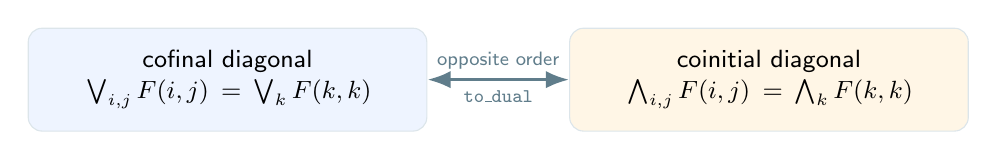
\begin{tikzpicture}[node distance=8mm and 18mm,>=Latex,
 n/.style={draw=line,rounded corners=5pt,text width=4.5cm,align=center,inner sep=8pt,font=\sffamily\small},
 ar/.style={<->,very thick,color=muted}]
 \node[n,fill=bluepale] (sup) {cofinal diagonal\\$\bigvee_{i,j}F(i,j)=\bigvee_kF(k,k)$};
 \node[n,fill=amberpale,right=of sup] (inf) {coinitial diagonal\\$\bigwedge_{i,j}F(i,j)=\bigwedge_kF(k,k)$};
 \draw[ar] (sup)--node[above,font=\sffamily\scriptsize]{opposite order}node[below,font=\ttfamily\scriptsize]{to\_dual} (inf);
\end{tikzpicture}
\end{center}

\vfill
{\color{muted}\scriptsize\sffamily Category theory explains the shape; the order-theoretic formulation supplies the weakest practical theorem.}

\newpage

% PAGE 6
{\sffamily\fontsize{23}{26}\selectfont\bfseries Structural insights for API design}\par
\vspace{3pt}
{\sffamily\color{muted}What this tiny lemma teaches beyond its three callers}\hfill\tagpill{tealpale}{DESIGN}

\vspace{11pt}
\begin{center}
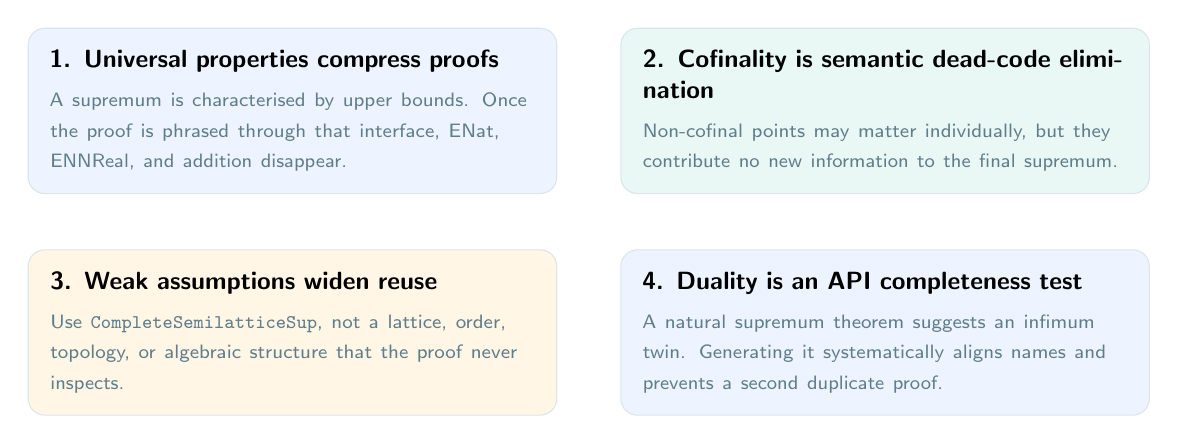
\begin{tikzpicture}[node distance=7mm and 8mm,>=Latex,
 insight/.style={draw=line,rounded corners=6pt,text width=6.15cm,minimum height=2.1cm,align=left,inner sep=8pt,font=\sffamily\small}]
 \node[insight,fill=bluepale] (a) {\textbf{1. Universal properties compress proofs}\\[3pt]
 \scriptsize\color{muted}A supremum is characterised by upper bounds. Once the proof is phrased through that interface, ENat, ENNReal, and addition disappear.};
 \node[insight,fill=tealpale,right=of a] (b) {\textbf{2. Cofinality is semantic dead-code elimination}\\[3pt]
 \scriptsize\color{muted}Non-cofinal points may matter individually, but they contribute no new information to the final supremum.};
 \node[insight,fill=amberpale,below=of a] (c) {\textbf{3. Weak assumptions widen reuse}\\[3pt]
 \scriptsize\color{muted}Use \texttt{CompleteSemilatticeSup}, not a lattice, order, topology, or algebraic structure that the proof never inspects.};
 \node[insight,fill=bluepale,below=of b] (d) {\textbf{4. Duality is an API completeness test}\\[3pt]
 \scriptsize\color{muted}A natural supremum theorem suggests an infimum twin. Generating it systematically aligns names and prevents a second duplicate proof.};
\end{tikzpicture}
\end{center}

\vspace{10pt}
\sectiontitle{The commutative proof picture}
\begin{center}
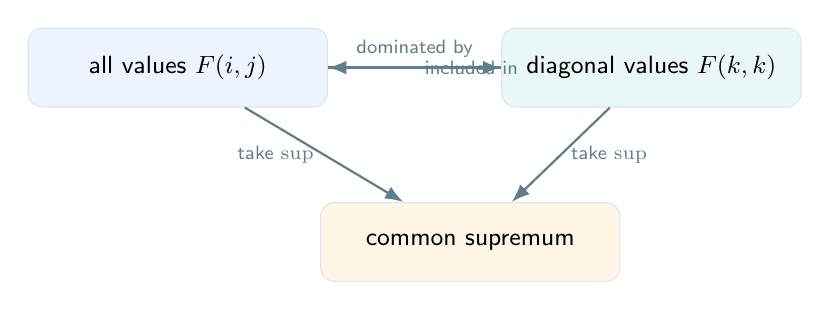
\begin{tikzpicture}[node distance=12mm and 22mm,>=Latex,
 n/.style={draw=line,rounded corners=5pt,fill=white,minimum width=3.8cm,minimum height=10mm,align=center,font=\sffamily\small},
 ar/.style={->,thick,color=muted}]
 \node[n,fill=bluepale] (grid) {all values $F(i,j)$};
 \node[n,fill=tealpale,right=of grid] (diag) {diagonal values $F(k,k)$};
 \node[n,fill=amberpale,below right=12mm and -1mm of grid] (sup) {common supremum};
 \draw[ar] (grid)--node[above,font=\sffamily\scriptsize]{dominated by} (diag);
 \draw[ar] (diag)--node[right,font=\sffamily\scriptsize]{included in} (grid);
 \draw[ar] (grid)--node[left,font=\sffamily\scriptsize]{take $\sup$} (sup);
 \draw[ar] (diag)--node[right,font=\sffamily\scriptsize]{take $\sup$} (sup);
\end{tikzpicture}
\end{center}

\vspace{8pt}
\begin{softbox}{tealpale}
{\sffamily\bfseries Two inequalities, two meanings}\par
\textbf{Inclusion} says the diagonal contributes no foreign values, so its supremum is no larger.\\
\textbf{Cofinality} says the omitted grid contributes no new height, so the full supremum is no larger.\\
Antisymmetry turns these complementary facts into equality.
\end{softbox}

\vspace{8pt}
\sectiontitle{A practical extraction checklist}
\begin{center}
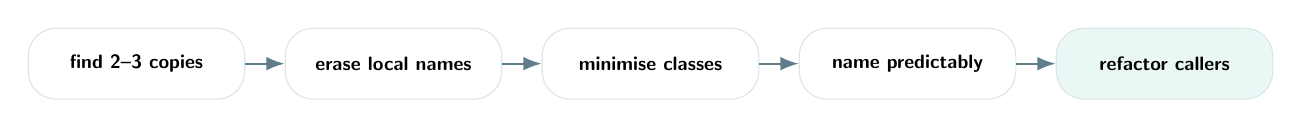
\begin{tikzpicture}[node distance=5mm and 5mm,>=Latex,
 c/.style={draw=line,rounded corners=10pt,fill=white,minimum width=2.75cm,minimum height=9mm,align=center,font=\sffamily\scriptsize\bfseries},
 ar/.style={->,thick,color=muted}]
 \node[c] (c1) {find 2--3 copies};
 \node[c,right=of c1] (c2) {erase local names};
 \node[c,right=of c2] (c3) {minimise classes};
 \node[c,right=of c3] (c4) {name predictably};
 \node[c,right=of c4,fill=tealpale] (c5) {refactor callers};
 \foreach \x/\y in {c1/c2,c2/c3,c3/c4,c4/c5} \draw[ar] (\x)--(\y);
\end{tikzpicture}
\end{center}

\vfill
{\color{muted}\scriptsize\sffamily The strongest contribution signal is not that a lemma can be proved, but that existing code becomes shorter and conceptually more uniform after it is named.}

\end{document}
